\section{Constant Coefficient Homogeneous Systems I}

\noindent
We'll now begin our study of the homogeneous system
\begin{equation}\label{eq:10.4.1}
{\bf y}'=A{\bf y},
\end{equation}
where $A$ is an $n\times n$ constant matrix. Since $A$ is continuous
on $(-\infty,\infty)$, Theorem~\ref{thmtype:10.2.1}
implies
that all solutions of \eqref{eq:10.4.1} are defined on $(-\infty,\infty)$.
Therefore, when we speak of solutions of ${\bf y}'=A{\bf y}$, we'll
mean solutions on $(-\infty,\infty)$.

In this section we assume that all the eigenvalues of $A$ are real and
that $A$ has a set of $n$ linearly independent eigenvectors. In the
next two sections we consider the cases where some of the eigenvalues
of $A$ are complex, or where $A$ does not have $n$ linearly
independent eigenvectors.

In Example~\ref{example:10.3.2} we showed that the vector
functions
$$
{\bf y}_1=\twocol {-e^{2t}}{2e^{2t}}\mbox{\quad and \quad}
{\bf y}_2=\twocol{-e^{-t}}{e^{-t}}
$$
form a fundamental set of solutions of the system
\begin{equation}\label{eq:10.4.2}
{\bf y}'=\twobytwo{-4}{-3}65 {\bf y},
\end{equation}
but we did not show how we obtained ${\bf y}_1$ and ${\bf y}_2$ in the
first place. To see how these solutions can be obtained we write
\eqref{eq:10.4.2} as
\begin{equation}\label{eq:10.4.3}
\begin{array}{ccc}
y_1'&=&-4y_1-3y_2\\y_2'&=&\phantom{-}6y_1+5y_2\end{array}
\end{equation}
and look for solutions of the form
\begin{equation}\label{eq:10.4.4}
y_1=x_1e^{\lambda t}\mbox{\quad and \quad}y_2=x_2e^{\lambda t},
\end{equation}
where $x_1$, $x_2$, and $\lambda$ are constants to be determined.
 Differentiating  \eqref{eq:10.4.4} yields
$$
y_1'=\lambda x_1e^{\lambda
t}\quad\mbox{ and }\quad y_2'=\lambda x_2e^{\lambda t}.
$$
Substituting this and  \eqref{eq:10.4.4} into  \eqref{eq:10.4.3} and canceling
the common factor $e^{\lambda t}$ yields
$$
\begin{array}{ccc}-4x_1-3x_2&=&\lambda x_1 \\
6 x_1+5x_2&=&\lambda x_2.\end{array}
$$
For a given $\lambda$, this is a homogeneous algebraic system, since it can
be rewritten as
\begin{equation}\label{eq:10.4.5}
\begin{array}{rcl} (-4-\lambda) x_1-3 x_2&=&0\\
6 x_1+(5-\lambda) x_2&=&0.\end{array}
\end{equation}
The trivial solution $x_1=x_2=0$ of this system isn't  useful, since
it corresponds to the trivial solution $y_1\equiv y_2\equiv0$ of
\eqref{eq:10.4.3}, which can't be part of a fundamental set of solutions
of \eqref{eq:10.4.2}. Therefore we consider only those values of $\lambda$
for which \eqref{eq:10.4.5} has nontrivial solutions. These are the values
of $\lambda$ for which the determinant of \eqref{eq:10.4.5} is zero;   that
is,
\begin{eqnarray*}
\left|\begin{array}{cc}-4-\lambda&-3\\6&5-\lambda\end{array}\right|&=&
(-4-\lambda)(5-\lambda)+18\\&=&\lambda^2-\lambda-2\\
&=&(\lambda-2)(\lambda+1)=0,
\end{eqnarray*}
which has the solutions $\lambda_1=2$ and $\lambda_2=-1$.

Taking $\lambda=2$ in  \eqref{eq:10.4.5} yields
\begin{eqnarray*}
-6 x_1-3 x_2&=&0\\
6 x_1+3 x_2&=&0,
\end{eqnarray*}
which implies that $x_1=-x_2/2$, where  $x_2$ can be
chosen arbitrarily. Choosing
$x_2=2$ yields the solution $y_1=-e^{2t}$,
$y_2=2e^{2t}$ of  \eqref{eq:10.4.3}. We can write this solution in vector
form as
\begin{equation}\label{eq:10.4.6}
{\bf y}_1=\twocol {-1}{\phantom{-}2} e^{2t}.
\end{equation}

Taking $\lambda=-1$ in  \eqref{eq:10.4.5} yields the system
\begin{eqnarray*}
-3 x_1-3 x_2&=&0\\
\phantom{-}6 x_1+6 x_2&=&0,
\end{eqnarray*}
so $x_1=-x_2$. Taking $x_2=1$ here
yields the solution $y_1=-e^{-t}$, $y_2=e^{-t}$ of  \eqref{eq:10.4.3}. We
can write this solution in vector form as
\begin{equation}\label{eq:10.4.7}
{\bf y}_2=\twocol{-1}{\phantom{-}1}e^{-t}.
\end{equation}

In \eqref{eq:10.4.6} and \eqref{eq:10.4.7} the constant coefficients in the
arguments of the exponential functions are the eigenvalues of the
coefficient matrix in \eqref{eq:10.4.2}, and the vector coefficients of the
exponential functions are associated eigenvectors. This illustrates
the next theorem.

\begin{theorem}\color{blue}\label{thmtype:10.4.1}
 Suppose the $n\times n$
constant matrix $A$ has $n$ real eigenvalues
$\lambda_1,\lambda_2,\ldots,\lambda_n$
{\rm(}which need not be distinct{\rm)} with associated
linearly independent eigenvectors ${\bf x}_1,{\bf x}_2,\ldots,{\bf x}_n$.
Then the functions
$$
{\bf y}_1={\bf x}_1e^{\lambda_1 t},\,
 {\bf y}_2={\bf x}_2e^{\lambda_2 t},\,
\dots,\,
{\bf y}_n={\bf x}_ne^{\lambda_n t}
$$
 form a fundamental set of solutions of  ${\bf y}'=A{\bf y};$
that is$,$ the general solution of this system is
$$
{\bf y}=c_1{\bf x}_1e^{\lambda_1 t}+c_2{\bf x}_2e^{\lambda_2 t}
+\cdots+c_n{\bf x}_ne^{\lambda_n t}.
$$
\end{theorem}

\proof
Differentiating ${\bf y}_i={\bf x}_ie^{\lambda_it}$ and recalling
that $A{\bf x}_i=\lambda_i{\bf x}_i$ yields
$$
{\bf y}_i'=\lambda_i{\bf x}_ie^{\lambda_it}=A{\bf x}_ie^{\lambda_it}
=A{\bf y}_i.
$$
This shows that ${\bf y}_i$ is a solution of ${\bf y}'=A{\bf y}$.

The Wronskian of
 $\{{\bf y}_1,{\bf y}_2,\ldots,{\bf y}_n\}$ is
$$
\left|\begin{array}{cccc}  x_{11}e^{\lambda_1 t}& x_{12}e^{\lambda_2
t}&\cdots& x_{1n}e^{\lambda_n t}\\
 x_{21}e^{\lambda_1 t}& x_{22}e^{\lambda_2
t}&\cdots& x_{2n}e^{\lambda_n t}\\\vdots&\vdots&\ddots&\vdots\\
  x_{n1}e^{\lambda_1 t}& x_{n2}e^{\lambda_2
t}&\cdots& x_{nn}e^{\lambda x_n t}\end{array}\right|
=e^{\lambda_1 t}e^{\lambda_2 t}\cdots e^{\lambda_n t}
\left|\begin{array}{cccc}
x_{11}&x_{12}&\cdots&x_{1n}\cr
\vspace{2\jot}
x_{21}&x_{22}&\cdots&x_{2n}\cr
\vspace{2\jot}
\vdots&\vdots&\ddots&\vdots\cr
\vspace{2\jot}
x_{n1}&x_{n2}&\cdots&x_{nn}\cr
\end{array}\right|.
$$
Since the columns of the determinant on the right are ${\bf x}_1$, ${\bf
x}_2$, \dots, ${\bf x}_n$, which are assumed to be linearly independent,
the determinant is nonzero. Therefore
Theorem~\ref{thmtype:10.3.3} implies that
$\{{\bf y}_1,{\bf y}_2,\ldots,{\bf y}_n\}$ is a fundamental set of
solutions of ${\bf y}'=A{\bf y}$.

\begin{example}\label{example:10.4.1}\rm
\mbox{}\newline
\begin{alist}
\item % (a)
 Find the general solution of
\begin{equation}\label{eq:10.4.8}
{\bf y}'=\twobytwo2442
{\bf y}.
\end{equation}

\item % (b)
 Solve the initial value problem
\begin{equation}\label{eq:10.4.9}
{\bf y}'=\twobytwo2442
{\bf y},\quad{\bf y}(0)=\left[\begin{array}{r}5 \\-1
\end{array}\right].
\end{equation}
\end{alist}
\end{example}

\solutionpart{a}   The characteristic
polynomial of the  coefficient matrix $A$ in  \eqref{eq:10.4.8} is
\begin{eqnarray*}
\left|\begin{array}{cc} 2-\lambda&4\\4&2-\lambda\end{array}\right|
&=& (\lambda-2)^2-16\\
&=& (\lambda-2-4)(\lambda-2+4)\\
&=& (\lambda-6)(\lambda+2).
\end{eqnarray*}
Hence,  $\lambda_1=6$ and $\lambda_2
=-2$ are eigenvalues of $A$. To obtain the eigenvectors,
we must solve the system
\begin{equation}\label{eq:10.4.10}
\left[\begin{array}{cc} 2-\lambda&4\\4&2-\lambda\end{array}\right]
\left[\begin{array}{c} x_1\\x_2\end{array}\right]=
\left[\begin{array}{c} 0\\0\end{array}\right]
\end{equation}
with $\lambda=6$ and $\lambda=-2$.  Setting $\lambda=6$ in
\eqref{eq:10.4.10} yields
 $$
\left[\begin{array}{rr}-4&4\\4&-4
\end{array}\right]\left[\begin{array}{c}
x_1\\x_2\end{array}\right]=\left[\begin{array}{c} 0\\0\end{array}
\right],
$$
which implies that $x_1=x_2$.  Taking $x_2=1$ yields the eigenvector
$$
{\bf x}_1=\left[\begin{array}{c} 1\\1\end{array}\right],
$$
so
$$
{\bf y}_1=\left[\begin{array}{c} 1\\1\end{array}\right]e^{6t}
$$
is a solution of  \eqref{eq:10.4.8}.  Setting $\lambda=-2$ in
\eqref{eq:10.4.10} yields
 $$
\left[\begin{array}{rr} 4&4\\4&4\end{array}\right]
\left[\begin{array}{c} x_1\\x_2
\end{array}\right]=\left[\begin{array}{c} 0\\0\end{array}\right],
$$
which implies that $x_1=-x_2$.  Taking $x_2=1$ yields the eigenvector
$$
{\bf x}_2=\left[\begin{array}{r}-1\\1\end{array}\right],
$$
so
$$
{\bf y}_2=\left[\begin{array}{r}-1\\1\end{array}
\right]e^{-2t}
$$
is a solution of  \eqref{eq:10.4.8}.
From Theorem~\ref{thmtype:10.4.1}, the general solution of
\eqref{eq:10.4.8} is
\begin{equation}\label{eq:10.4.11}
{\bf y}=c_1{\bf y}_1+c_2{\bf y}_2=c_1\left[\begin{array}{r}1\\1
\end{array}\right]e^{6t}+c_2\left[\begin{array}{r}-1\\1
\end{array}\right]e^{-2t}.
\end{equation}

\solutionpart{b}
 To satisfy the initial condition in  \eqref{eq:10.4.9}, we must choose
$c_1$ and $c_2$ in  \eqref{eq:10.4.11} so that
$$
c_1\left[\begin{array}{r}1\\1\end{array}\right]+c_2\left[
\begin{array}{r}-1\\
1\end{array}\right]=\left[\begin{array}{r}5\\-1
\end{array}\right].
$$
This is equivalent to the system
\begin{eqnarray*}
c_1-c_2&=&\phantom{-}5\\
c_1+c_2&=&-1,
\end{eqnarray*}
so $c_1=2, c_2=-3$.  Therefore the solution of
\eqref{eq:10.4.9} is
$$
{\bf y}=2\left[\begin{array}{r}1\\1\end{array}\right]e^{6t}-3
\left[\begin{array}{r}-1\\1\end{array}\right]e^{-2t},
$$
or, in terms of components,
$$
y_1=2e^{6t}+3e^{-2t},\quad y_2=2e^{6t}-3e^{-2t}.
$$

\begin{example}\label{example:10.4.2} \rm
\mbox{}\newline
\begin{alist}
\item % (a)
 Find the general solution of
\begin{equation}\label{eq:10.4.12}
{\bf y}'=\left[\begin{array}{rrr}3&-1&-1\\-2&
3&
2\\4&-1&-2\end{array}\right]{\bf y}.
\end{equation}

\item  % (b)
 Solve the initial value problem
\begin{equation}\label{eq:10.4.13}
{\bf y}'=\left[\begin{array}{rrr}3&-1&-1\\-2&3&
2\\4&-1&-2\end{array}
\right]{\bf y},\quad{\bf y}(0)=\left[\begin{array}{r}2\\
-1\\8\end{array}\right].
\end{equation}
\end{alist}
\end{example}

\solutionpart{a}   The characteristic
polynomial of the  coefficient matrix $A$ in  \eqref{eq:10.4.12} is
$$
\left|\begin{array}{ccc}3-\lambda&-1&-1\\-2&3-\lambda&
2\\4
&-1&-2-\lambda\end{array}\right|=-(\lambda-2)(\lambda-3)(\lambda+1).
$$
Hence, the eigenvalues of $A$ are $\lambda_1=2$, $\lambda_2=3$,  and
$\lambda_3=-1$.
To find the  eigenvectors, we must solve the system
\begin{equation}\label{eq:10.4.14}
\left[\begin{array}{ccc}3-\lambda&-1&-1\\-2&3-\lambda&
2\\4&-1&
-2-\lambda\end{array}\right]\left[\begin{array}{c} x_1\\x_2\\x_3
\end{array}
\right]=\left[\begin{array}{r}0\\0\\0\end{array}\right]
\end{equation}
with $\lambda=2$, $3$, $-1$.  With $\lambda=2$, the augmented matrix of
\eqref{eq:10.4.14} is
$$
\left[\begin{array}{rrrcr} 1&-1&-1&\vdots&0\\-2&
1&2&\vdots&0\\4&-1&-4&\vdots&0
\end{array}\right],
$$
which is row equivalent to
$$
\left[\begin{array}{rrrcr} 1&0&-1&\vdots&0\\0&1&0&
\vdots&0\\0&0&0&\vdots&0\end{array}\right].
$$
Hence,  $x_1=x_3$ and $x_2=0$.  Taking $x_3=1$ yields
$$
{\bf y}_1=\left[\begin{array}{rrr}1\\0\\1\end{array}\right]e^{2t}
$$
as a solution of  \eqref{eq:10.4.12}.  With $\lambda=3$, the augmented
matrix of  \eqref{eq:10.4.14} is
$$
\left[\begin{array}{rrrcr}0&-1&-1&\vdots&0\\-2&
0& 2&\vdots&0\\4&-1&-5&\vdots&0
\end{array}\right],
$$
which is row equivalent to
$$
\left[\begin{array}{rrrcr} 1&0&-1&\vdots&0\\0&1&1&
\vdots&0\\0&0&0&\vdots&0\end{array}\right].
$$
Hence,  $x_1=x_3$ and $x_2=-x_3$. Taking $x_3=1$ yields
$$
{\bf y}_2=\left[\begin{array}{r}1\\-1\\1\end{array}
\right]e^{3t}
$$
as a solution of  \eqref{eq:10.4.12}.  With $\lambda=-1$, the augmented
matrix of  \eqref{eq:10.4.14} is
$$
\left[\begin{array}{rrrcr} 4&-1&-1&\vdots&0\\-2&4&
2&\vdots&0\\4&-1&-1&\vdots&0
\end{array}\right],
$$
which is row equivalent to
$$
\left[\begin{array}{rrrcr} 1&0&-{1\over 7}&\vdots&0\\0&1&
{3\over
7}&\vdots&0\\0&0&0&\vdots&0\end{array}\right].
$$
Hence, $x_1=x_3/7$ and $x_2=-3x_3/7$.  Taking $x_3=7$ yields
$$
{\bf y}_3=\left[\begin{array}{r}1\\-3\\7\end{array}
\right]e^{-t}
$$
as a solution of  \eqref{eq:10.4.12}. By Theorem~\ref{thmtype:10.4.1},
 the general solution of  \eqref{eq:10.4.12} is
$$
{\bf y}=c_1\left[\begin{array}{r}1\\0\\1\end{array}\right]e^{2t}
+c_2\left[\begin{array}{r}1\\-1\\1\end{array}\right]
e^{3t}+c_3
\left[\begin{array}{r}1\\-3\\7\end{array}\right]e^{-t},
$$
which can also be written as
\begin{equation}\label{eq:10.4.15}
{\bf y}=\left[\begin{array}{crc}e^{2t}&e^{3t}&e^{-t}
\\0&-e^{3t}&
-3e^{-t}\\e^{2t}&e^{3t}&\phantom{-}7e^{-t}\end{array}
\right]\left[\begin{array}{c} c_1\\c_2\\c_3\end{array}\right].
\end{equation}

\solutionpart{b}
 To satisfy the initial condition in  \eqref{eq:10.4.13} we must choose
$c_1$, $c_2$, $c_3$ in  \eqref{eq:10.4.15} so that
$$
\left[\begin{array}{rrr}1&1&1\\0&-1&-3\\
1&1&7\end{array}\right]
\left[\begin{array}{c} c_1\\c_2\\c_3\end{array}\right]=
\left[\begin{array}{r}2\\-1\\8\end{array}\right].
$$
Solving this system yields $c_1=3$, $c_2=-2$, $c_3=1$.  Hence, the solution
of  \eqref{eq:10.4.13} is
\begin{eqnarray*}
{\bf y}&=&\left[\begin{array}{ccc}e^{2t}&e^{3t}&
e^{-t}\\0&-e^{3t}
&-3e^{-t}\\e^{2t}&e^{3t}&7e^{-t}\end{array}
\right]
\left[\begin{array}{r}3\\-2\\1\end{array}\right]\\
&=&3\left[\begin{array}{r}1\\0\\1\end{array}\right]e^{2t}-2
\left[\begin{array}{r}1\\-1\\1\end{array}\right]
e^{3t}+\left[\begin{array}{r}1\\-3\\7\end{array}
\right]e^{-t}.
\end{eqnarray*}

\begin{example}\label{example:10.4.3}\rm
 Find the general solution of
\begin{equation}\label{eq:10.4.16}
{\bf y}'=\left[\begin{array}{rrr}-3&2&2\\
2&-3&2\\2&2&-3
\end{array}\right]{\bf y}.
\end{equation}
\end{example}

\solution  The characteristic polynomial of
the  coefficient matrix $A$ in  \eqref{eq:10.4.16} is
$$
\left|\begin{array}{ccc}-3-\lambda&2&2\\2&-3-\lambda&2\\2&2
&-3-\lambda\end{array}\right|=-(\lambda-1)(\lambda+5)^2.
$$
Hence, $\lambda_1=1$ is an eigenvalue of multiplicity $1$, while
$\lambda_2=-5$ is an eigenvalue of multiplicity $2$. Eigenvectors
associated with $\lambda_1=1$ are solutions of the system with
augmented matrix
$$
\left[\begin{array}{rrrcr}-4&2&2&\vdots&0\\
2
&-4&2&\vdots&0\\2&2&-4&
\vdots&0\end{array}\right], $$
which is row equivalent to
$$
\left[\begin{array}{rrrcr} 1&0&-1&\vdots& 0\\0&1&-1 &\vdots& 0
\\0&0&0&\vdots&0\end{array}\right].
$$
Hence, $x_1=x_2=x_3$, and we choose $x_3=1$ to obtain the solution
\begin{equation}\label{eq:10.4.17}
{\bf y}_1=\left[\begin{array}{r}1\\1\\1\end{array}\right]e^t
\end{equation}
of  \eqref{eq:10.4.16}.  Eigenvectors associated with $\lambda_2=-5$
are solutions of the system
with  augmented matrix
$$
\left[\begin{array}{rrrcr} 2&2&2&\vdots&0\\2&2&2&\vdots&0
\\2&2&2&\vdots&0\end{array}\right].
$$
Hence, the components of these eigenvectors need only satisfy the single
condition
$$
x_1+x_2+x_3=0.
$$
Since there's only one equation here, we can choose $x_2$ and
$x_3$  arbitrarily. We obtain one eigenvector by choosing $x_2=0$
and $x_3=1$, and another by choosing $x_2=1$ and $x_3=0$. In both
cases $x_1=-1$. Therefore
$$
\left[\begin{array}{r}-1\\0\\1\end{array}\right]\quad
\mbox{ and }\quad\left[\begin{array}{r}-1\\1\\0
\end{array}\right]
$$
are linearly independent eigenvectors associated with  $\lambda_2=
-5$, and the corresponding solutions of  \eqref{eq:10.4.16} are
$$
{\bf y}_2=\left[\begin{array}{r}-1\\0\\1\end{array}
\right]e^{-5t}\quad
\mbox{ and }\quad{\bf y}_3=\left[\begin{array}{r}-1\\1\\
0\end{array}\right]e^{-5t}.
$$
Because of this and  \eqref{eq:10.4.17}, Theorem~\ref{thmtype:10.4.1} implies
that  the general solution of \eqref{eq:10.4.16} is
$$
{\bf y}=c_1\left[\begin{array}{r}1\\1\\
1\end{array}\right]e^t+c_2
\left[\begin{array}{r}-1\\0\\1\end{array}\right]
e^{-5t}+c_3\left[\begin{array}{r}-1\\1\\0\end{array}
\right]e^{-5t}.
 $$

\boxit{Geometric Properties of Solutions when  $n=2$}

\noindent
We'll now  consider the geometric properties of solutions of a
$2\times2$ constant coefficient system
\begin{equation} \label{eq:10.4.18}
\twocol{y_1'}{y_2'}=\left[\begin{array}{cc}a_{11}&a_{12}\\a_{21}&a_{22}
\end{array}\right]\twocol{y_1}{y_2}.
\end{equation}
It is convenient to think of a ``$y_1$-$y_2$ plane," where a point
is identified by rectangular coordinates $(y_1,y_2)$. If ${\bf
y}=\dst{\twocol{y_1}{y_2}}$ is a non-constant solution of \eqref{eq:10.4.18},
then the point $(y_1(t),y_2(t))$ moves along a curve $C$ in the
$y_1$-$y_2$ plane as $t$ varies from $-\infty$ to $\infty$. We call
$C$ the {\color{blue}\it trajectory\/} of ${\bf y}$. (We also say that $C$ is a
trajectory of the system \eqref{eq:10.4.18}.) I's important to note that
$C$ is the trajectory of infinitely many solutions of \eqref{eq:10.4.18},
since if $\tau$ is any real number, then ${\bf y}(t-\tau)$ is a
solution of \eqref{eq:10.4.18} (Exercise~\ref{exer:10.4.28}(b)), and
$(y_1(t-\tau),y_2(t-\tau))$ also moves along $C$ as $t$ varies from
$-\infty$ to $\infty$. Moreover, Exercise~\ref{exer:10.4.28}\part{c}
implies
that distinct trajectories of \eqref{eq:10.4.18} can't intersect, and that
two solutions ${\bf y}_1$ and ${\bf y}_2$ of \eqref{eq:10.4.18} have the
same trajectory if and only if ${\bf y}_2(t)={\bf y}_1(t-\tau)$ for
some $\tau$.

From Exercise~\ref{exer:10.4.28}\part{a}, a trajectory of a nontrivial
solution
of \eqref{eq:10.4.18} can't contain $(0,0)$, which we define to be the
trajectory of the trivial solution ${\bf y}\equiv0$. More generally,
if ${\bf y}=\dst{\twocol{k_1}{k_2}}\ne{\bf 0}$ is a constant solution
of \eqref{eq:10.4.18} (which could occur if zero is an eigenvalue of the
matrix of \eqref{eq:10.4.18}), we define the trajectory of ${\bf y}$ to be
the single point $(k_1,k_2)$.

To be specific, this is the question: What do the trajectories look
like, and how are they traversed? In this section we'll answer this
question, assuming that the matrix
$$
A=\left[\begin{array}{cc}a_{11}&a_{12}\\a_{21}&a_{22}
\end{array}\right]
$$
of \eqref{eq:10.4.18} has real eigenvalues $\lambda_1$ and $\lambda_2$ with
associated linearly independent eigenvectors ${\bf x}_1$ and ${\bf
x}_2$. Then  the general solution of \eqref{eq:10.4.18} is
\begin{equation} \label{eq:10.4.19}
{\bf y}= c_1{\bf x}_1
 e^{\lambda_1 t}+c_2{\bf x}_2e^{\lambda_2 t}.
\end{equation}
We'll consider other situations in the next two sections.

We leave it to you (Exercise~\ref{exer:10.4.35}) to classify the
trajectories of \eqref{eq:10.4.18} if zero is an eigenvalue of $A$. We'll
confine our attention here to the case where both eigenvalues are
nonzero. In this case the simplest situation is where
$\lambda_1=\lambda_2\ne0$, so  \eqref{eq:10.4.19} becomes
$$
{\bf y}=(c_1{\bf x}_1+c_2{\bf x}_2)e^{\lambda_1 t}.
$$
Since ${\bf x}_1$ and
${\bf x}_2$ are linearly independent, an arbitrary vector ${\bf x}$
can be written as ${\bf x}=c_1{\bf x}_1+c_2{\bf x}_2$. Therefore the
general solution of \eqref{eq:10.4.18} can be written as ${\bf y}={\bf
x}e^{\lambda_1 t}$ where ${\bf x}$ is an arbitrary $2$-vector, and the
trajectories of nontrivial solutions of \eqref{eq:10.4.18} are half-lines
through (but not including) the origin. The direction of motion is
away from the origin if $\lambda_1>0$ (Figure~\ref{figure:10.4.1}),
toward it if $\lambda_1<0$ (Figure~\ref{figure:10.4.2}). (In these
and the next figures an arrow through a point indicates the
direction of motion along the trajectory through the point.)

\begin{figure}[H]
\color{blue}
  \begin{minipage}[b]{0.5\linewidth}
    \centering
   \scalebox{.65}{
  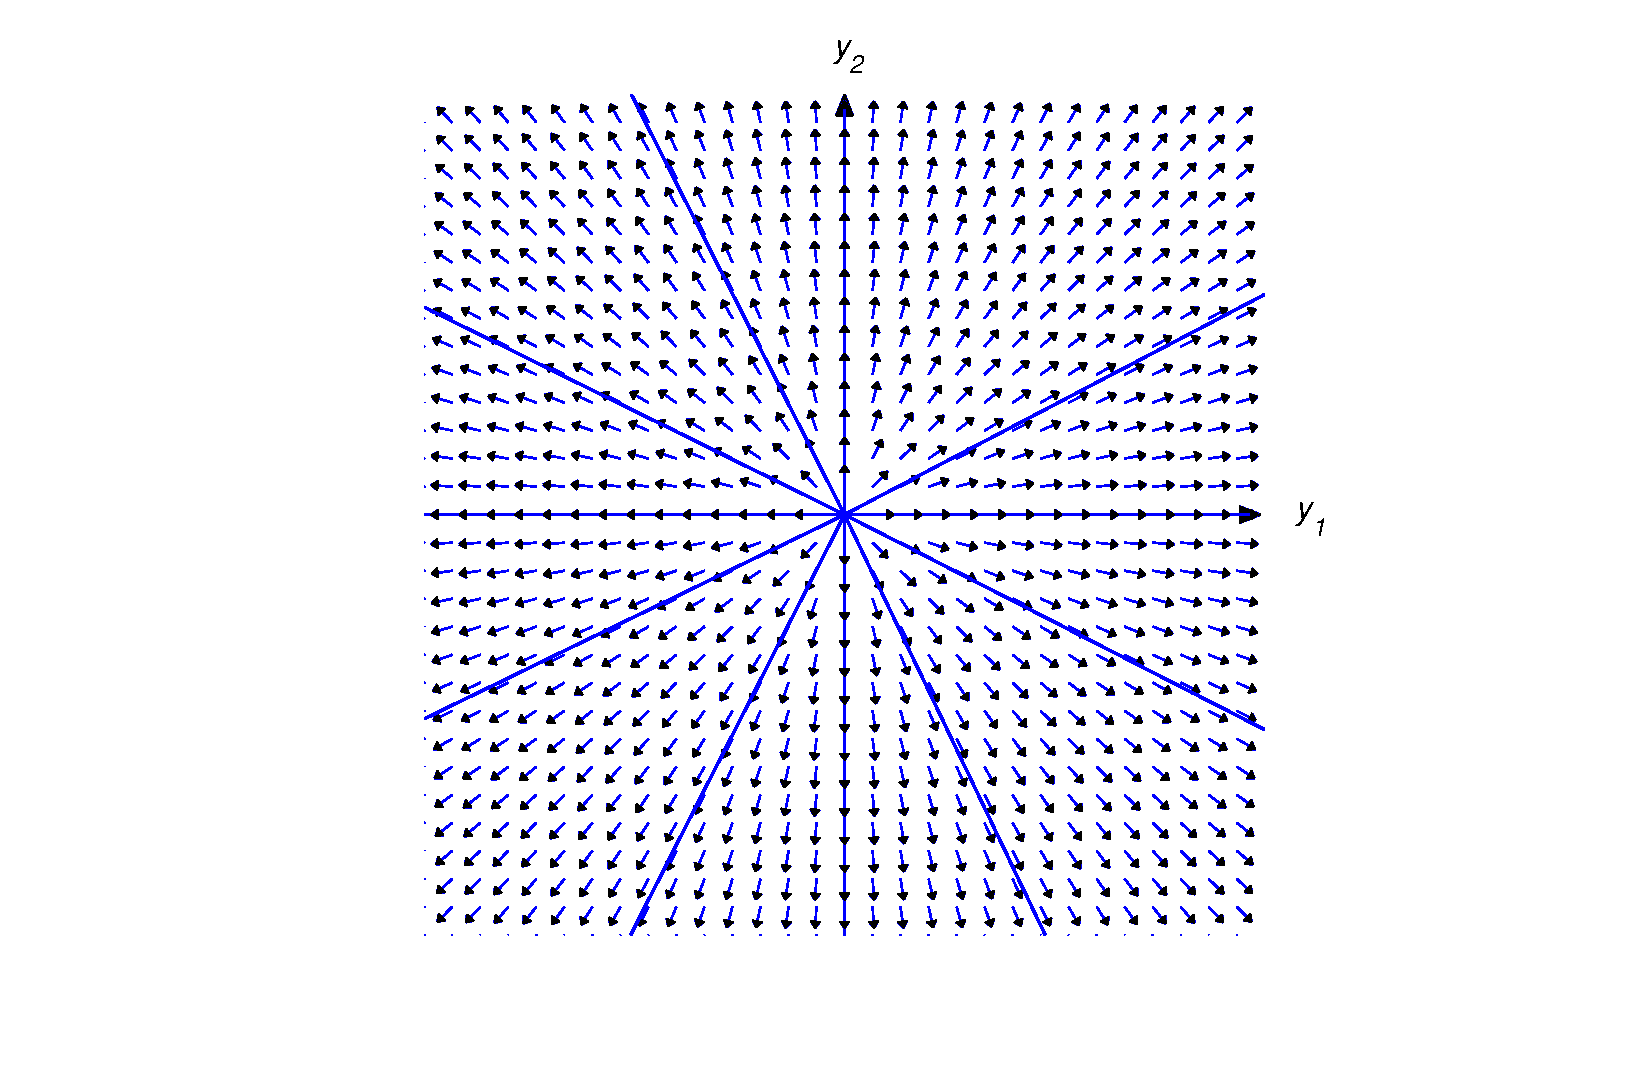
\includegraphics[bb=-78 148 689 643,width=5.67in,height=3.66in,keepaspectratio]{fig100401}}
\caption{
Trajectories of a $2\times2$ system with a repeated positive
eigenvalue}
  \label{figure:10.4.1}
\end{minipage}
  \begin{minipage}[b]{0.5\linewidth}
    \centering
   \scalebox{.65}{
  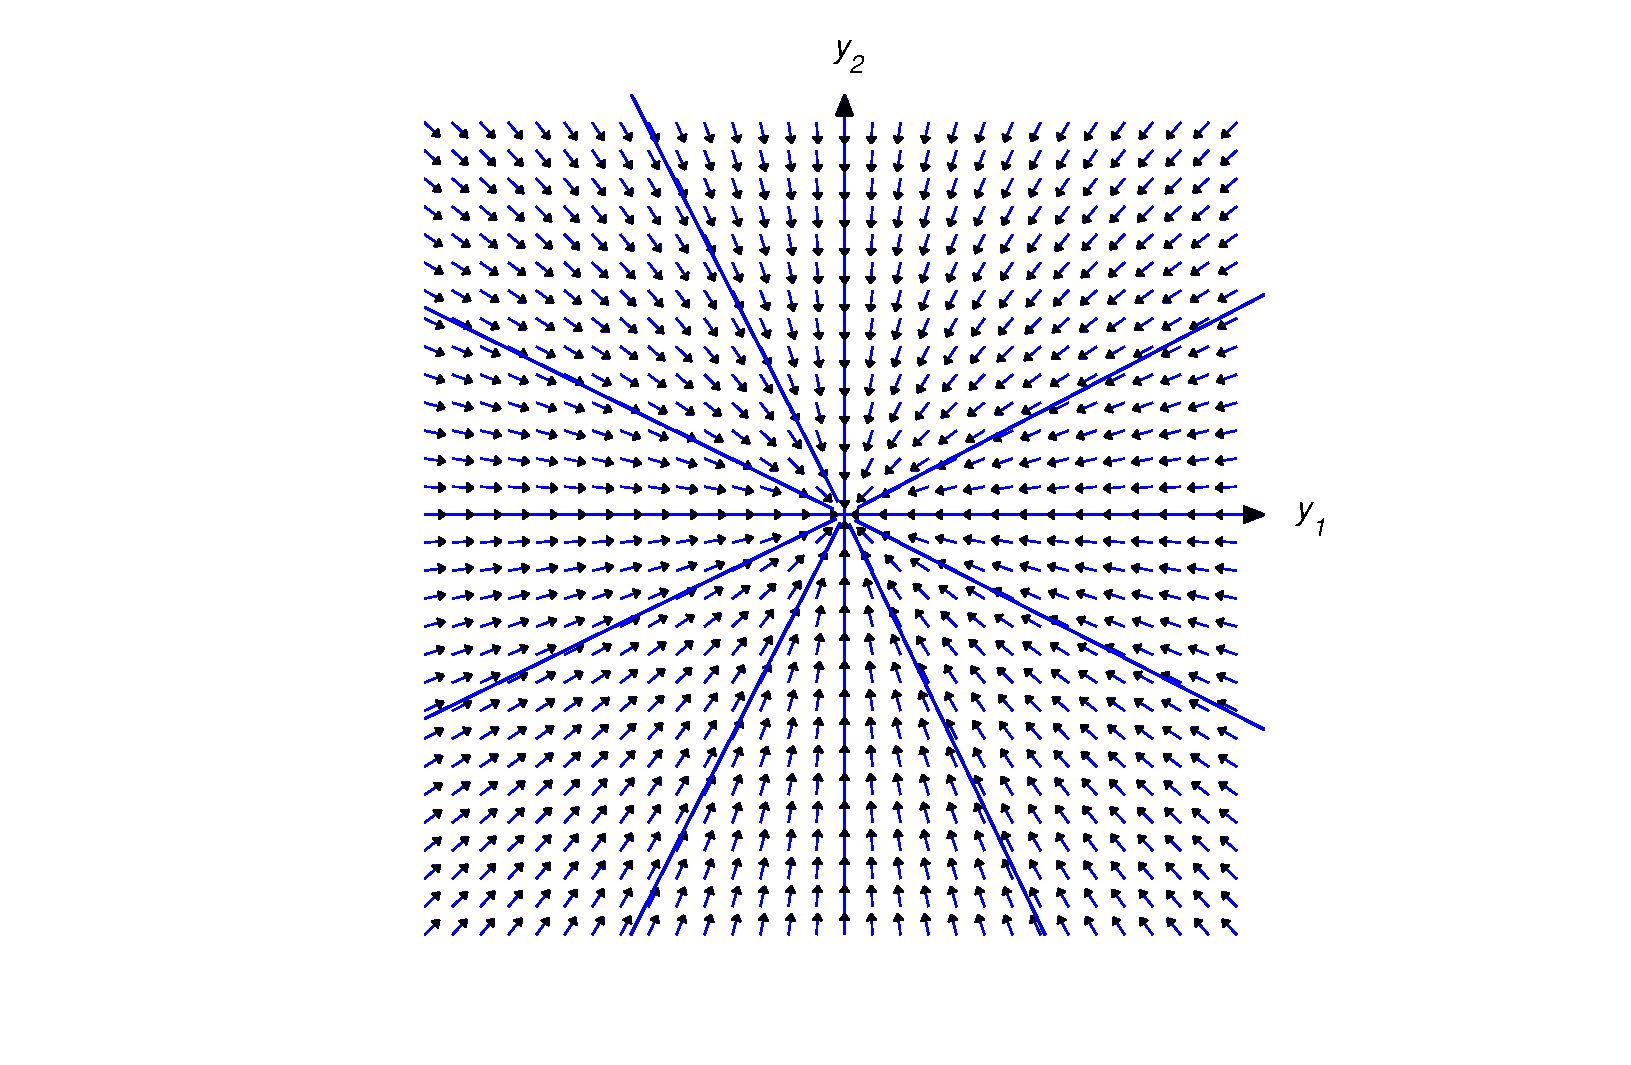
\includegraphics[bb=-78 148 689 643,width=5.67in,height=3.66in,keepaspectratio]{fig100402}}
\caption{
Trajectories of a $2\times2$ system with a repeated negative
eigenvalue}
  \label{figure:10.4.2}
\end{minipage}
\end{figure}

Now suppose   $\lambda_2>\lambda_1$, and let $L_1$ and $L_2$ denote
lines through the origin parallel to ${\bf x}_1$ and ${\bf x}_2$,
respectively. By a half-line of $L_1$ (or $L_2$), we mean either of the
rays obtained by removing the origin from $L_1$ (or $L_2$).

Letting $c_2=0$ in \eqref{eq:10.4.19} yields ${\bf y}=c_1{\bf
x}_1e^{\lambda_1 t}$. If $c_1\ne0$, the trajectory defined by this
solution is a half-line of $L_1$. The direction of motion is away from
the origin if $\lambda_1>0$, toward the origin if $\lambda_1<0$.
Similarly, the trajectory of  ${\bf y}=c_2{\bf x}_2e^{\lambda_2 t}$
with $c_2\ne0$ is a half-line of $L_2$.

Henceforth, we assume that $c_1$ and $c_2$ in \eqref{eq:10.4.19} are both
nonzero. In this case, the trajectory of \eqref{eq:10.4.19} can't
intersect
$L_1$ or $L_2$, since every point on these lines is on the trajectory
of a solution for which either $c_1=0$ or $c_2=0$. (Remember: distinct
trajectories can't intersect!). Therefore the trajectory of
\eqref{eq:10.4.19} must lie entirely in one of the four open sectors
bounded by $L_1$ and $L_2$, but do not any point  on $L_1$ or
$L_2$. Since the initial point $(y_1(0),y_2(0))$ defined by
$$
{\bf y}(0)=c_1{\bf x}_1+c_2{\bf x}_2
$$
is on the trajectory, we can determine which sector contains the
trajectory from the signs of $c_1$ and $c_2$,
as shown in Figure~\ref{figure:10.4.3}.

The direction of ${\bf y}(t)$ in \eqref{eq:10.4.19} is the
same as that of
\begin{equation} \label{eq:10.4.20}
e^{-\lambda_2 t}{\bf y}(t)=
c_1{\bf x}_1e^{-(\lambda_2-\lambda_1)t}+c_2{\bf x}_2
\end{equation}
and of
\begin{equation} \label{eq:10.4.21}
e^{-\lambda_1 t}{\bf y}(t)=c_1{\bf
x}_1+c_2{\bf x}_2e^{(\lambda_2-\lambda_1)t}.
\end{equation}
Since the right side of \eqref{eq:10.4.20} approaches $c_2{\bf x}_2$ as
$t\to\infty$, the trajectory is asymptotically parallel to $L_2$ as
$t\to\infty$. Since the right side of \eqref{eq:10.4.21} approaches
$c_1{\bf x}_1$ as $t\to-\infty$, the trajectory is asymptotically
parallel to $L_1$ as $t\to-\infty$.

The shape and direction of
traversal of the trajectory of \eqref{eq:10.4.19} depend upon whether
$\lambda_1$ and $\lambda_2$ are both positive, both negative, or of
opposite signs. We'll now analyze these three cases.

Henceforth $\|{\bf u}\|$  denote the length of the vector
${\bf u}$.

\begin{figure}[htbp]
\color{blue}
  \begin{minipage}[b]{0.5\linewidth}
    \centering
   \scalebox{.65}{
  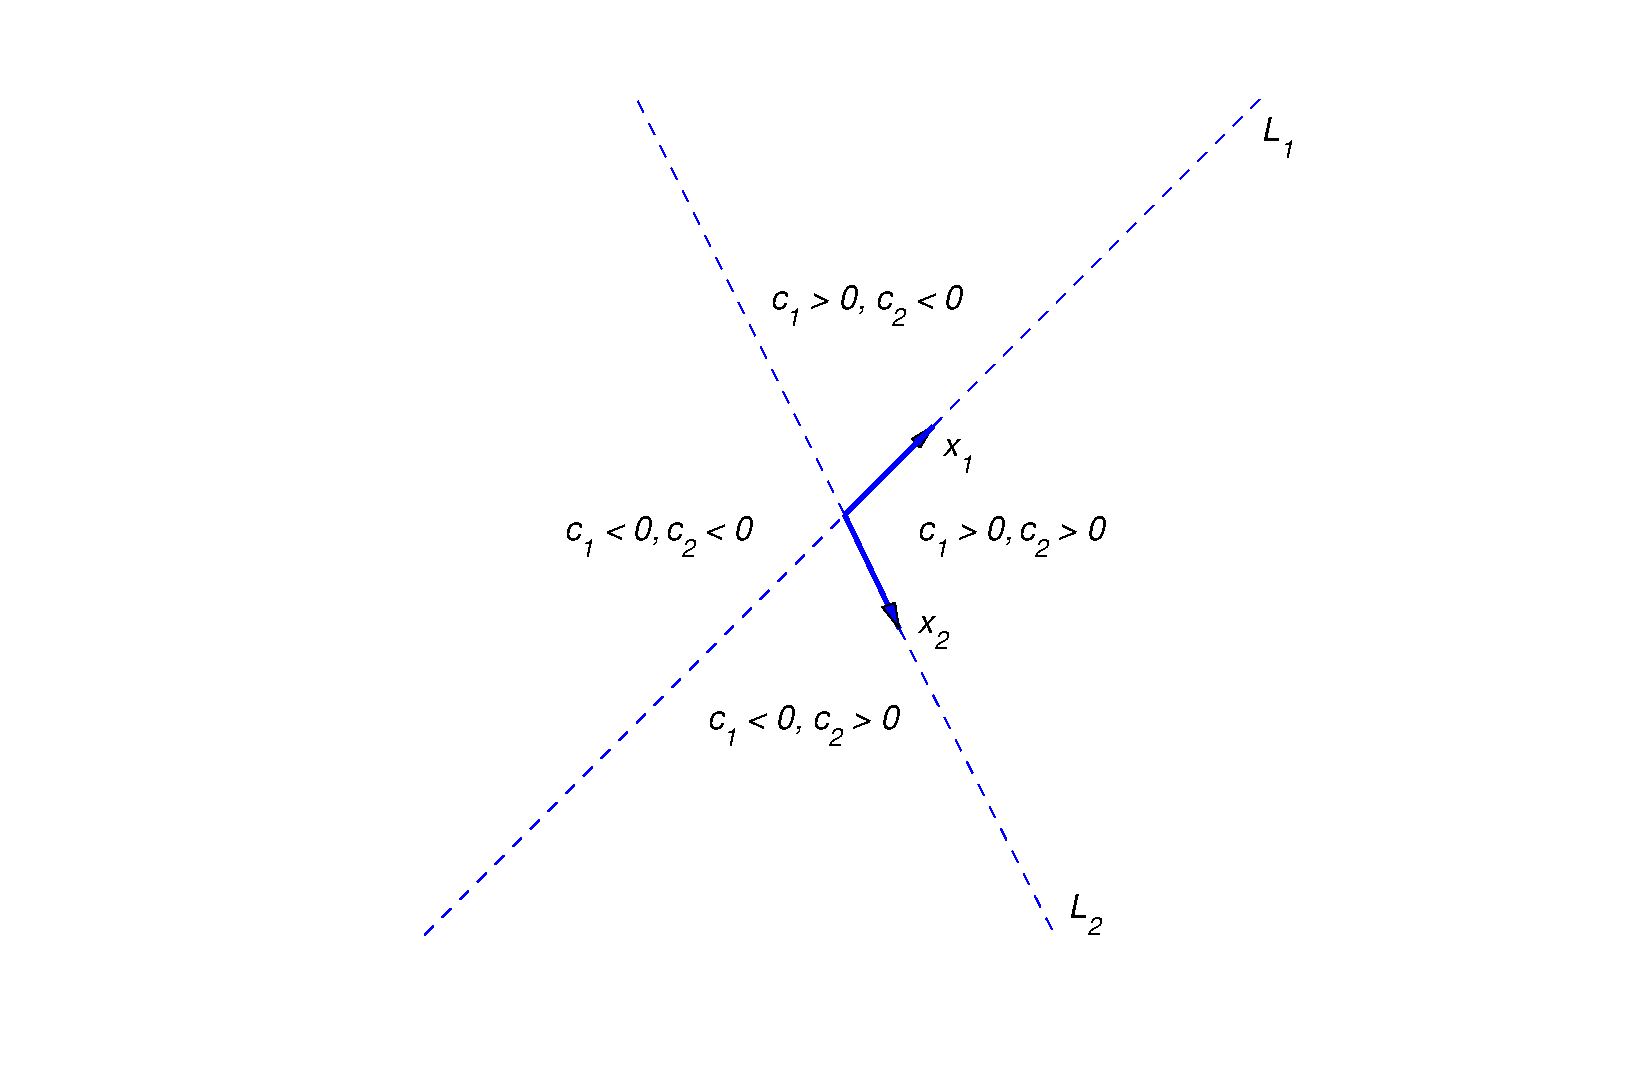
\includegraphics[bb=-78 148 689 643,width=5.67in,height=3.66in,keepaspectratio]{fig100403} }
  \caption{ Four open sectors bounded by $L_1$ and $L_2$}
  \label{figure:10.4.3}
\end{minipage}
  \begin{minipage}[b]{0.5\linewidth}
    \centering
   \scalebox{.65}{
  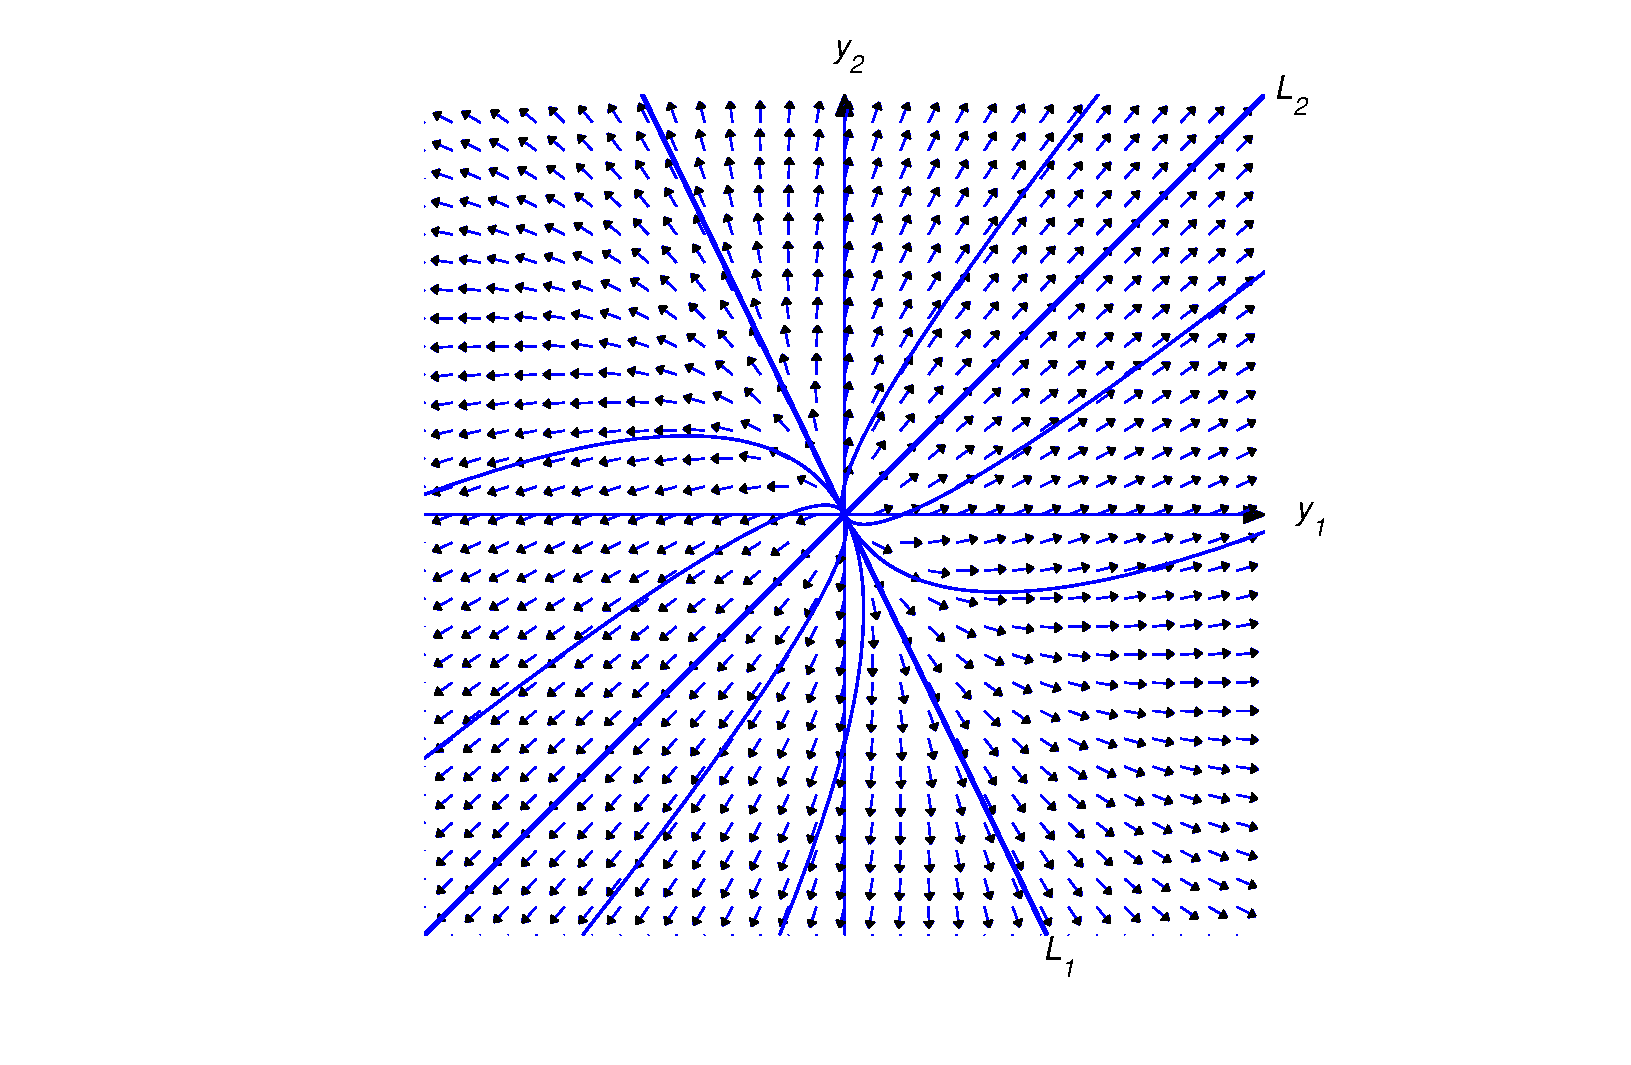
\includegraphics[bb=-78 148 689 643,width=5.67in,height=3.66in,keepaspectratio]{fig100404}  }
\caption{ Two positive eigenvalues;   motion away from
origin}
  \label{figure:10.4.4}
\end{minipage}
\end{figure}

\boxit{Case 1: $\lambda_2>\lambda_1>0$}

\noindent
Figure~\ref{figure:10.4.4}  shows some
 typical trajectories.
In this case, $\lim_{t\to-\infty}\|{\bf y}(t)\|=0$, so the trajectory
is not only asymptotically parallel to $L_1$ as $t\to-\infty$, but is
actually asymptotically tangent to $L_1$ at the origin. On
the other hand, $\lim_{t\to\infty}\|{\bf y}(t)\|=\infty$ and
$$
\lim_{t\to\infty}\left\|{\bf y}(t)-c_2{\bf x}_2e^{\lambda_2
t}\right\|=\lim_{t\to\infty}\|c_1{\bf x_1}e^{\lambda_1t}\|=\infty,
$$
so, although the trajectory is asymptotically parallel to $L_2$ as
$t\to\infty$, it's not asymptotically tangent to $L_2$.
The direction of motion along each trajectory is away from the origin.

\boxit{Case 2: $0>\lambda_2>\lambda_1$}

\noindent
Figure~\ref{figure:10.4.5}   shows
some typical trajectories.
In this case, $\lim_{t\to\infty}\|{\bf y}(t)\|=0$, so the trajectory is
asymptotically tangent to $L_2$ at the origin as $t\to\infty$. On the
other hand, $\lim_{t\to-\infty}\|{\bf y}(t)\|=\infty$ and
$$
\lim_{t\to-\infty}\left\|{\bf y}(t)-c_1{\bf x}_1e^{\lambda_1
t}\right\|=\lim_{t\to-\infty}\|c_2{\bf x}_2e^{\lambda_2t}\|=\infty,
$$
so, although the trajectory is asymptotically parallel to $L_1$ as
$t\to-\infty$, it's not asymptotically tangent to it.
The direction of motion along each trajectory is toward the origin.

\begin{figure}[htbp]
\color{blue}
  \begin{minipage}[b]{0.5\linewidth}
    \centering
   \scalebox{.65}{
  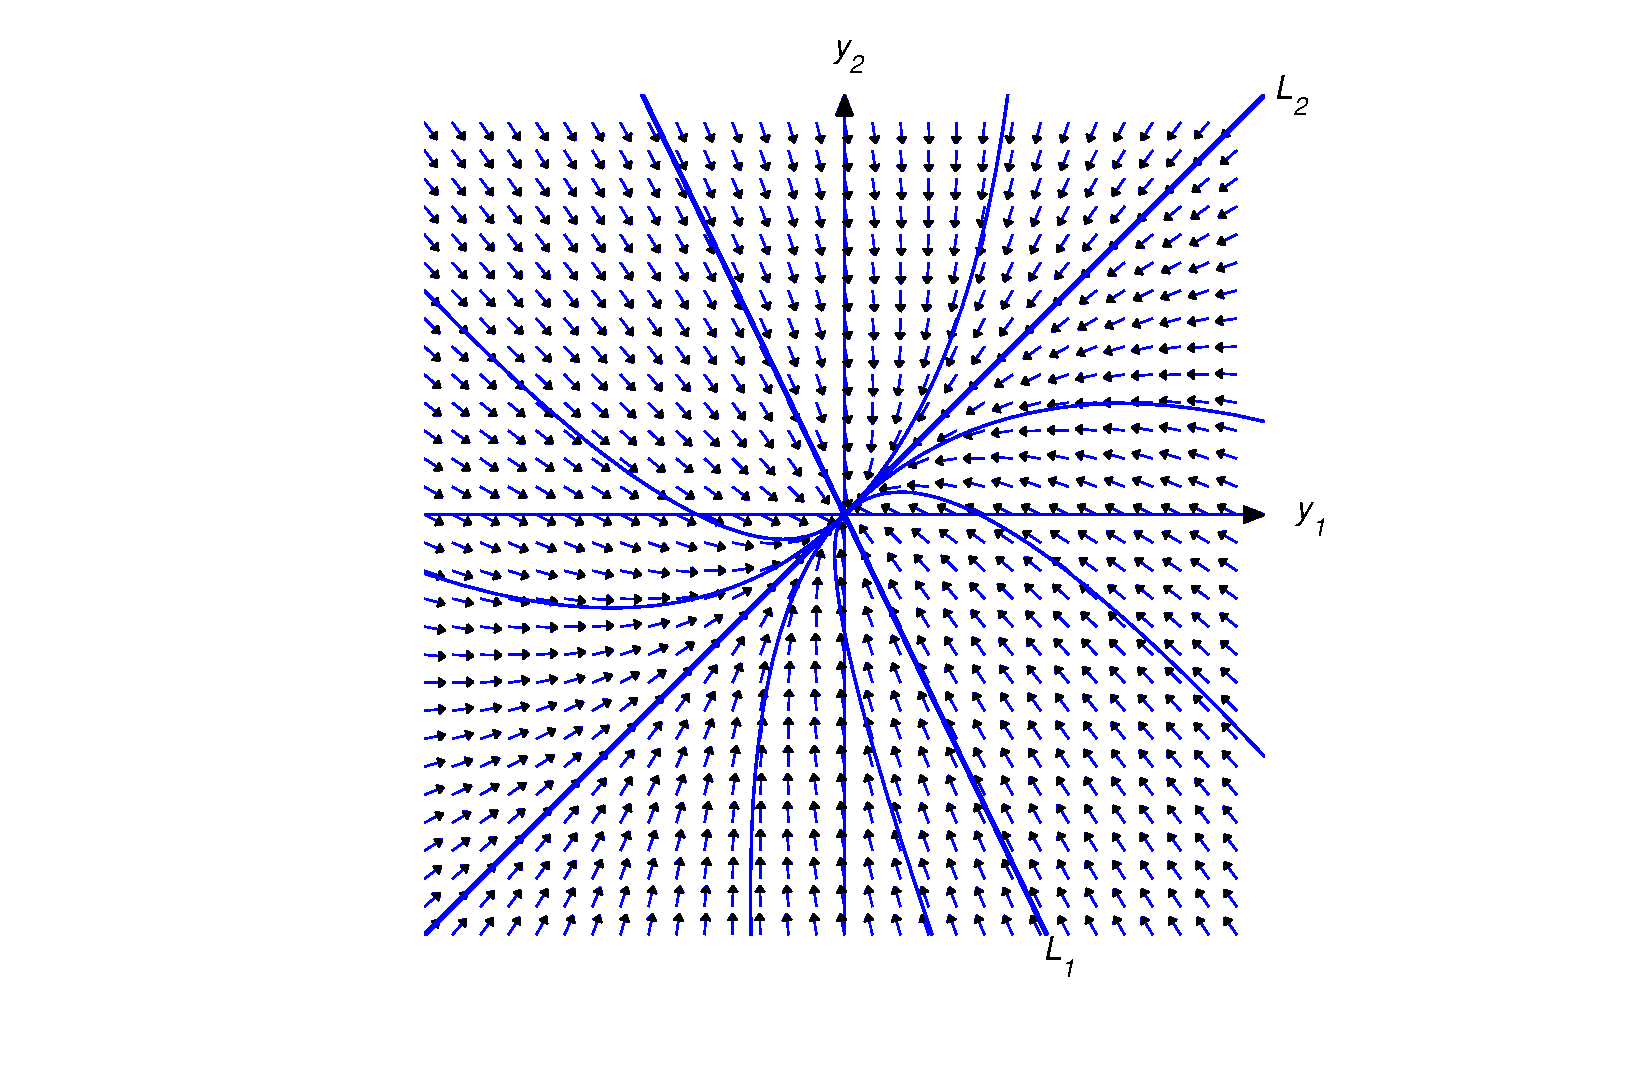
\includegraphics[bb=-78 148 689 643,width=5.67in,height=3.66in,keepaspectratio]{fig100405} }
\caption{
 Two negative eigenvalues;   motion toward the origin}
  \label{figure:10.4.5}
\end{minipage}
  \begin{minipage}[b]{0.5\linewidth}
    \centering
   \scalebox{.65}{
  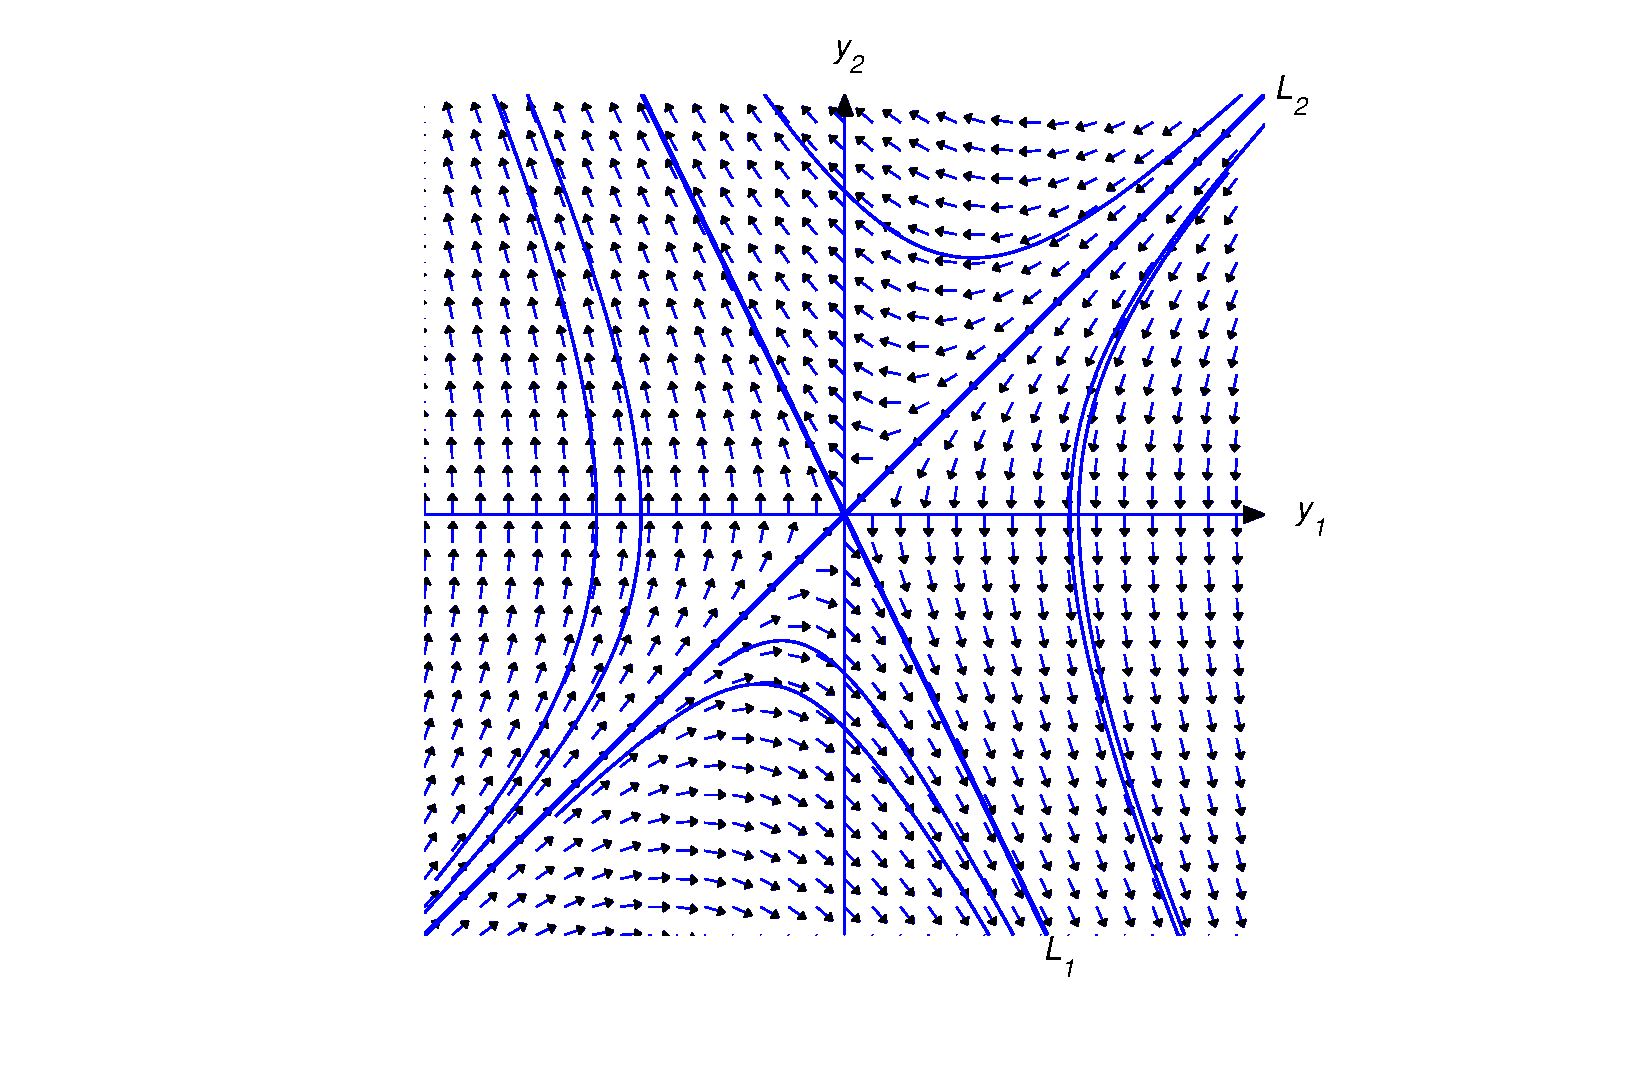
\includegraphics[bb=-78 148 689 643,width=5.67in,height=3.66in,keepaspectratio]{fig100406}}
\caption{ Eigenvalues of different signs}
  \label{figure:10.4.6}
\end{minipage}
\end{figure}

\boxit{Case 3: $\lambda_2>0>\lambda_1$}

\noindent
Figure~\ref{figure:10.4.6} shows
some typical trajectories.
In this case,
$$
\lim_{t\to\infty}\|{\bf y}(t)\|=\infty \mbox{\quad and \quad}
\lim_{t\to\infty}\left\|{\bf y}(t)-c_2{\bf x}_2e^{\lambda_2
t}\right\|=\lim_{t\to\infty}\|c_1{\bf x}_1e^{\lambda_1t}\|=0,
$$
so the trajectory is asymptotically tangent to $L_2$ as $t\to\infty$.
Similarly,
$$
\lim_{t\to-\infty}\|{\bf y}(t)\|=\infty \mbox{\quad and \quad}
\lim_{t\to-\infty}\left\|{\bf y}(t)-c_1{\bf x}_1e^{\lambda_1
t}\right\|=\lim_{t\to-\infty}\|c_2{\bf x}_2e^{\lambda_2t}\|=0,
$$
so the trajectory is asymptotically tangent to $L_1$ as $t\to-\infty$.
The direction of motion is toward the origin on $L_1$ and away from
the origin on $L_2$. The direction of motion along any other
trajectory is away from $L_1$, toward $L_2$.

\exercises
 In Exercises~\ref{exer:10.4.1}--\ref{exer:10.4.15} find the general
solution.

\begin{exerciselist}
\begin{tabular}[t]{@{}p{168pt}@{}p{168pt}}
\item\label{exer:10.4.1} $\dst{{\bf y}'=
\left[\begin{array}{rr} 1&2\\2&1\end{array}\right]{\bf y}}$&
\item\label{exer:10.4.2} $\dst{{\bf y}'=
{1\over4}\left[\begin{array}{rr}-5&3 \\3&-5\end{array}\right]{\bf
y}}$
\end{tabular}

\begin{tabular}[t]{@{}p{168pt}@{}p{168pt}}
\item\label{exer:10.4.3} $\dst{{\bf y}'=
{1\over5}\left[\begin{array}{rr}-4&3\\
-2&-11\end{array}\right]{\bf y}}$&
\item\label{exer:10.4.4} $\dst{{\bf y}'=
\left[\begin{array}{rr}-1&-4\\-1&-1\end{array}\right]{\bf y}}$
\end{tabular}

\begin{tabular}[t]{@{}p{168pt}@{}p{168pt}}
\item\label{exer:10.4.5} $\dst{{\bf y}'=
\left[\begin{array}{rr} 2&-4\\-1&-1\end{array}\right]{\bf y}}$&
\item\label{exer:10.4.6} $\dst{{\bf y}'=
\left[\begin{array}{rr} 4&-3\\2&-1\end{array}\right]{\bf y}}$
\end{tabular}

\begin{tabular}[t]{@{}p{168pt}@{}p{168pt}}
\item\label{exer:10.4.7} $\dst{{\bf y}'=
\left[\begin{array}{rr}-6&-3\\1&-2\end{array}\right]{\bf y}}$&
\item\label{exer:10.4.8} $\dst{{\bf y}'=
\left[\begin{array}{rrr}
1&-1&-2\\1&-2&-3\\-4&1&-1\end{array}\right]
{\bf y}}$
\end{tabular}

\begin{tabular}[t]{@{}p{168pt}@{}p{168pt}}
\item\label{exer:10.4.9} $\dst{{\bf y}'=
\left[\begin{array}{rrr}
-6&-4&-8\\-4&0&-4\\-8&-4&-6\end{array}\right]{\bf y}}$&
\item\label{exer:10.4.10} $\dst{{\bf y}'=
\left[\begin{array}{rrr}3&5&8\\1&-1&
-2\\-1&-1&-1\end{array}\right]{\bf y}}$
\end{tabular}

\begin{tabular}[t]{@{}p{168pt}@{}p{168pt}}
\item\label{exer:10.4.11}  $\dst{{\bf y}'=
\left[\begin{array}{rrr}
1&-1&2\\12&-4
& 10\\-6&1&-7
\end{array}\right]{\bf y}}$&
\item\label{exer:10.4.12} $\dst{{\bf y}'=
\left[\begin{array}{rrr}
4&-1&-4\\4&-3&-2\\1&-1&-1\end{array}\right]{\bf y}}$
\end{tabular}

\begin{tabular}[t]{@{}p{168pt}@{}p{168pt}}
\item\label{exer:10.4.13} $\dst{{\bf y}'=
\left[\begin{array}{rrr}-2&2&-6\\2&6&2\\-2&-2&
2\end{array}\right]{\bf y}}$&
\item\label{exer:10.4.14} $\dst{{\bf y}'=
\left[\begin{array}{rrr}3&2&-2\\-2&7&-2\\
-10&10&-5\end{array}\right]{\bf y}}$ \end{tabular}

\item\label{exer:10.4.15} $\dst{{\bf y}'=
\left[\begin{array}{rrr}3&1&-1\\3&5&1\\-6&2&4\end{array}
\right]{\bf y}}$

\exercisetext{In Exercises~\ref{exer:10.4.16}--\ref{exer:10.4.27}
solve the initial value problem.}

\item\label{exer:10.4.16}
$\dst{{\bf y}'=\twobytwo{-7}4{-6}7{\bf y},\quad{\bf
y}(0)=\twocol2{-4}}$

\item\label{exer:10.4.17}
$\dst{{\bf y}'={1\over6}\twobytwo72{-2}2{\bf y},\quad{\bf
y}(0)=\twocol0{-3}}$

\item\label{exer:10.4.18}
$\dst{{\bf y}'=\twobytwo{21}{-12}{24}{-15}{\bf y},\quad{\bf
y}(0)=\twocol53}$

\item\label{exer:10.4.19}
$\dst{{\bf y}'=\twobytwo{-7}4{-6}7{\bf y},\quad{\bf
y}(0)=\twocol{-1}7}$

\item\label{exer:10.4.20}
$\dst{{\bf y}'={1\over6}\threebythree1204{-1}0003{\bf y},\quad{\bf
y}(0)=\threecol471}$

\item\label{exer:10.4.21}
$\dst{{\bf y}'={1\over3}\threebythree2{-2}3{-4}43210{\bf
y},\quad{\bf y}(0)=\threecol115}$

\item\label{exer:10.4.22}
$\dst{{\bf y}'=\threebythree6{-3}{-8}21{-2}3{-3}{-5}{\bf
y},\quad{\bf y}(0)=\threecol0{-1}{-1}}$

\item\label{exer:10.4.23}
$\dst{{\bf y}'={1\over3}\threebythree24{-7}15{-5}{-4}4{-1}{\bf
y},\quad{\bf y}(0)=\threecol413}$

\item\label{exer:10.4.24} $\dst{
{\bf y}'=\threebythree301{11}{-2}7103{\bf y},\quad
{\bf y}(0)=\threecol276}$

\item\label{exer:10.4.25} $\dst{
{\bf y}'=\threebythree{-2}{-5}{-1}{-4}{-1}145{3}{\bf y},\quad
{\bf y}(0)=\threecol8{-10}{-4}}$

\item\label{exer:10.4.26}  $\dst{
{\bf y}'=\threebythree3{-1}04{-2}04{-4}2{\bf y},\quad
{\bf y}(0)=\threecol7{10}2}$

\item\label{exer:10.4.27} $\dst{{\bf y}'=
\left[\begin{array}{rrr}-2&2&6\\2&6&2\\-2&-2&
2\end{array}\right]{\bf y}},\quad{\bf y}(0)=\threecol6{-10}7$

\item\label{exer:10.4.28}
Let $A$ be an $n\times n$ constant matrix. Then
Theorem~\ref{thmtype:10.2.1} implies that the solutions
of
$$
{\bf y}'=A{\bf y}
\eqno{\rm(A)}
$$
are all defined on $(-\infty,\infty)$.
\begin{alist}
\item % (a)
Use Theorem~\ref{thmtype:10.2.1} to show that the only
solution
of (A) that can ever equal the zero vector is ${\bf y}\equiv{\bf0}$.
\item % (b)
Suppose ${\bf y}_1$ is a solution of (A) and ${\bf y}_2$ is
defined by ${\bf y}_2(t)={\bf y}_1(t-\tau)$, where $\tau$ is an
arbitrary real number. Show that ${\bf y}_2$ is also a solution of
(A).
\item % (c)
Suppose ${\bf y}_1$ and ${\bf y}_2$ are solutions of (A) and
there are real numbers $t_1$ and $t_2$ such that ${\bf y}_1(t_1)={\bf
y}_2(t_2)$. Show that ${\bf y}_2(t)={\bf y}_1(t-\tau)$ for all $t$,
where $\tau=t_2-t_1$. \hint{Show that ${\bf y}_1(t-\tau)$ and ${\bf
y}_2(t)$ are solutions of the same initial value problem for {\rm
(A)},
and apply the uniqueness assertion of
Theorem~\ref{thmtype:10.2.1}.}
\end{alist}

\exercisetext{In Exercises~\ref{exer:10.4.29}-~\ref{exer:10.4.34}
describe and graph trajectories of the given system.}

\begin{tabular}[t]{@{}p{168pt}@{}p{168pt}}
\item\label{exer:10.4.29} \CGex ${\bf y}'=\dst{\twobytwo111{-1}}{\bf y}$&
\item\label{exer:10.4.30} \CGex ${\bf y}'=\dst{\twobytwo{-4}3{-2}{-11}}{\bf
y}$
\end{tabular}

\begin{tabular}[t]{@{}p{168pt}@{}p{168pt}}
\item\label{exer:10.4.31} \CGex ${\bf y}'=\dst{\twobytwo9{-3}{-1}{11}}{\bf
y}$&
\item\label{exer:10.4.32} \CGex ${\bf
y}'=\dst{\twobytwo{-1}{-10}{-5}4}{\bf y}$
\end{tabular}

\begin{tabular}[t]{@{}p{168pt}@{}p{168pt}}
\item\label{exer:10.4.33} \CGex ${\bf y}'=\dst{\twobytwo5{-4}1{10}}{\bf
y}$&
\item\label{exer:10.4.34} \CGex ${\bf
y}'=\dst{\twobytwo{-7}13{-5}}{\bf y}$
\end{tabular}

\item\label{exer:10.4.35}
Suppose the eigenvalues of the $2\times 2$
matrix $A$ are $\lambda=0$ and $\mu\ne0$, with
corresponding  eigenvectors ${\bf x}_1$ and ${\bf x}_2$.
Let $L_1$ be the line through the origin parallel to ${\bf x}_1$.
\begin{alist}
\item % (a)
Show that every point on $L_1$ is the trajectory of a constant
solution of ${\bf y}'=A{\bf y}$.
\item % (b)
Show that the trajectories of nonconstant solutions of ${\bf y}'=A{\bf
y}$ are half-lines parallel to ${\bf x}_2$ and on either side of
$L_1$, and that the direction of motion along these trajectories is
away from $L_1$ if $\mu>0$, or toward $L_1$ if $\mu<0$.
\end{alist}

\exercisetext{The matrices of the systems in
Exercises~\ref{exer:10.4.36}-\ref{exer:10.4.41} are singular. Describe
and graph the trajectories of nonconstant solutions  of the given
systems.}

\begin{tabular}[t]{@{}p{168pt}@{}p{168pt}}
\item\label{exer:10.4.36} \CGex ${\bf y}'=\dst{\twobytwo{-1}11{-1}}{\bf y}$&
\item\label{exer:10.4.37} \CGex ${\bf y}'=\dst{\twobytwo{-1}{-3}26}{\bf
y}$
\end{tabular}

\begin{tabular}[t]{@{}p{168pt}@{}p{168pt}}
\item\label{exer:10.4.38} \CGex ${\bf y}'=\dst{\twobytwo1{-3}{-1}3}{\bf
y}$&
\item\label{exer:10.4.39} \CGex ${\bf y}'=\dst{\twobytwo1{-2}{-1}2}{\bf y}$
\end{tabular}

\begin{tabular}[t]{@{}p{168pt}@{}p{168pt}}
\item\label{exer:10.4.40} \CGex ${\bf y}'=\dst{\twobytwo{-4}{-4}11}{\bf
y}$&
\item\label{exer:10.4.41} \CGex ${\bf
y}'=\dst{\twobytwo3{-1}{-3}1}{\bf y}$
\end{tabular}

\item\label{exer:10.4.42} \Lex
Let $P=P(t)$ and $Q=Q(t)$ be the populations of two species at time
$t$, and assume that each population would grow exponentially if the
other didn't exist; that is, in the absence of competition,
$$
P'=aP \mbox{\quad and \quad}Q'=bQ,
\eqno{\rm(A)}
$$
where $a$ and $b$ are positive constants. One way to model the effect
of competition is to assume that the growth rate per individual of
each population is reduced by an amount proportional to the other
population, so (A) is replaced by
\begin{eqnarray*}
P'&=&\phantom{-}aP-\alpha Q\\
Q'&=&-\beta P+bQ,
\end{eqnarray*}
where $\alpha$ and $\beta$ are positive constants. (Since negative
population doesn't make sense, this system holds only while $P$ and
$Q$ are both positive.) Now suppose $P(0)=P_0>0$ and
$Q(0)=Q_0>0$.

\begin{alist}
\item % (a)
For several choices of $a$, $b$, $\alpha$, and $\beta$, verify
experimentally
(by graphing trajectories of (A) in the $P$-$Q$ plane) that there's a
constant $\rho>0$ (depending upon $a$, $b$, $\alpha$, and $\beta$) with the
following properties:
\begin{rmlist}
\item % (i)
If $Q_0>\rho P_0$, then $P$ decreases monotonically to zero
in finite time, during which $Q$ remains positive.
\item % (ii)
If $Q_0<\rho P_0$, then $Q$ decreases monotonically to zero in
finite time, during which $P$ remains positive.
\end{rmlist}
\item % (b)
Conclude from  \part{a} that exactly one of the species
becomes extinct in finite time if $Q_0\ne\rho P_0$. Determine
experimentally what happens if $Q_0=\rho P_0$.
\item % (c)
Confirm your experimental results and determine $\gamma$ by expressing
the eigenvalues and associated eigenvectors of
$$
A=\twobytwo a{-\alpha}{-\beta}b
$$
in terms of $a$, $b$, $\alpha$, and $\beta$, and applying the geometric
arguments developed at the end of this section.
\end{alist}

\end{exerciselist}
